 \section{Einleitung}
 Speicherprogrammierbare Steuerungen oder kurz SPS tauchen überall dort auf, wo große elektrische Maschinen eingesetzt werden. Dies ist vor allem in der Industrie der Fall. Ihr kleiner Bruder ist die Kleinsteuerung. Sie bietet die selben Kernfunktionen, hat jedoch eine deutlich kleinere Anzahl an Ein- und Ausgängen. Sie werden häufig von Elektroinstallateuren eingesetzt, wenn eine klassische verbindungsprogrammierte Steuerung zum Beispiel durch Drahtbruch oder defekte Spulen in eingesetzten Relais nicht mehr korrekt funktionieren. Der Hersteller Eaton hat mit seinem Produkt \chphl{Easy} (siehe \autoref{img:EatonEasy}) genau diese Zielgruppe im Blick. Die Programmierung erfolgt hier, als würde man klassische Schütz-Kontakte in Reihe schalten. Die Einstiegsgeräte sind relativ preiswert, doch kauft man sich in eine proprietäre Produktwelt ein, welche aufgrund von inkompatiblen Bauteilen und Bussystemen schwer wieder zu verlassen ist. So gestaltet sich die Erweiterung einer bestehenden Steuerung um die Möglichkeit einer Fernabfrage übers Internet als nahezu unmöglich, oder setzt den Austausch der kompletten Steuerung voraus. Dabei sind Ein- und Ausgänge doch eigentlich das selbe wie an jedem Raspberry Pi vorhandene GPIOs. Auf Basis dieser Überlegung und günstigen Preisen hierfür, entstand die Idee eine Lösung mittels Raspberry Pi zu erarbeiten. 
 
  \begin{figure}[H]
 	\begin{center}
 		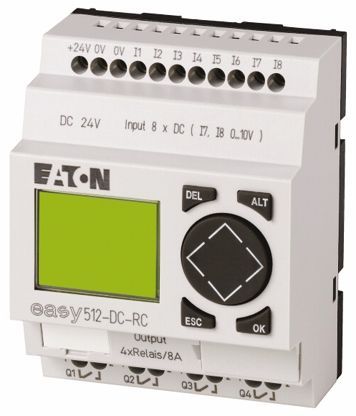
\includegraphics[width=0.5\textwidth]{./images/Easy.jpg}
 		\caption[Eaton Easy Kleinsteuerung]{Eaton Easy Kleinsteuerung \cite{URL:EatonEasy}}
 		\label{img:EatonEasy}
 	\end{center} 
 \end{figure}	
 
\subsection{Ziel der Arbeit}
Ziel dieser Arbeit ist es dabei vor allem eine möglichst günstige Möglichkeit zu schaffen um eine Steuerung zu realisieren, welche intuitiv programmiert werden kann und die Grundsätzliche Funktion der vorher eingesetzten Easy Steuerung um die Möglichkeit zur Fernabfrage übers Internet und weitere Funktionen erweitert. Dabei soll das Projekt mittels Git \cite{BOOK:GIT} versioniert werden um es anderen Entwicklern auf GitHub als Open-Source Software zur Verfügung zu stellen. Dabei wird das Projekt als MIT lizenziert, was eine Modifikation sowie private und gewerbliche Nutzung und Verbreitung ausdrücklich gestattet. 
\subsection{Verwandte Arbeiten}
Bei der Recherche nach weiteren Projekten, welche auf Basis eines Raspberry Pi eine Speicherprogrammierbare Steuerung realisieren, fand sich zum einen das kommerzielle Projekt Codesys \cite{URL:Codesys}. Auch zu nennen ist das Projekt Open-PLC \cite{URL:OpenPLC}. 
\subsection{Aufbau der Arbeit}
In dieser Arbeit werden zunächst einige grundsätzliche Fragen der Steuerungstechnik thematisiert. Hierbei wird besprochen weshalb eine Speicherprogrammierbare Steuerung überhaupt benötigt wird, wie man sie einsetzt und wie die gängige Praxis zum Erstellen von Steuerungsprogrammen ist. Weiterhin werden einige eingesetzte Technologien in Hard- und Software beschrieben. Zuletzt wird auch auf einige organisatorische Dinge, wie die Versionsverwaltung oder die Entwicklungsumgebung eingegangen. Kapitel \chphl{\ref{kap:ums} \nameref{kap:ums}} beschreibt dann, wie die Arbeit praktisch umgesetzt wurde und geht dabei auf die logische Unterteilung der Komponenten sowie deren Zusammenspiel und die darin eingesetzten Algorithmen ein. Das letzte Kapitel beschreibt bis wohin die Entwicklung gelangt ist und welche Fehler noch bestehen. Außerdem wird hier darauf eingegangen wie die ordnungsgemäße Funktion überprüft werden kann und weißt auf mögliche Szenarien hin, die zu Fehlern führen könnten. Im Anhang bietet sich ein Überblick über die beigelegte DVD. Außerdem lassen sich die Softwareversionen der eingesetzten Tools hier nachlesen.

\clearpage
